\documentclass[tikz]{standalone}
\usepackage{pgfplots}
\pgfplotsset{compat=1.18}
\definecolor{utnblue}{RGB}{0, 102, 204}

\begin{document}
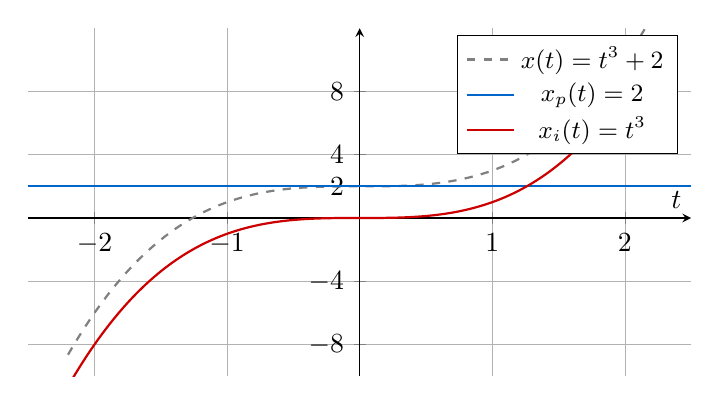
\begin{tikzpicture}
    \begin{axis}[
        width=10cm, height=6cm,
        axis lines=middle,
        xmin=-2.5, xmax=2.5, ymin=-10, ymax=12,
        xlabel={$t$}, ylabel={},
        grid=both,
        grid style={line width=.1pt, draw=gray!40},
        major grid style={line width=.2pt, draw=gray!60},
        xtick={-2,-1,0,1,2},
        ytick={-8,-4,0,2,4,8},
        samples=200,
        domain=-2.2:2.2,
        legend style={at={(0.98,0.98)}, anchor=north east, font=\small},
        every axis plot/.append style={thick},
    ]
    % Señal original t^3 + 2
    \addplot[gray, dashed] {x^3 + 2};
    \addlegendentry{$x(t) = t^3 + 2$}
    % Componente par = 2
    \addplot[utnblue] coordinates {(-2.5,2) (2.5,2)};
    \addlegendentry{$x_p(t) = 2$}
    % Componente impar = t^3
    \addplot[red!80!black] {x^3};
    \addlegendentry{$x_i(t) = t^3$}
    \end{axis}
\end{tikzpicture}
\end{document}
